%\documentclass[11pt,twoside]{eitExjobb}
\documentclass[11pt,twoside,final]{eitExjobb}  % Use final for the final version that will be printed
%%%%%%%%%%%%%%%%%%%%%%%%%%%%%%%%%%%%%%%%%%%%%%%%%%%%
%% Other fonts (Palatino as rm font, helvetica as sf font and courier as tt font. All fonts are normally installed with a standard LaTeX distribution.)
% \usepackage{mathpazo} % Also in math mode
% \usepackage[scaled=.95]{helvet}
% \usepackage{courier}
%%%%%%%%%%%%%%%%%%%%%%%%%%%%%
% Double spacing
\usepackage{setspace}

% svg usage
\usepackage{svg}
\usepackage{pdfpages}

% To use subfigures
\usepackage{subcaption}

\usepackage{multirow}
\usepackage{amsmath}
\usepackage{array}
\usepackage{hhline}

\usepackage[utf8]{inputenc}  % Input encoding (this file): 8 bit unicode. Default by most text editors
\usepackage[T1]{fontenc}     % Output encoding (pdf file)
%%%%%%%%%%%%%%%%%%%%%%%%%%%%%
%% Packages used in the example

%\usepackage{graphicx}   % Included graphics and some resizable boxes
%\usepackage{url}        % nice urls with line breaks
%\usepackage{lipsum}     % nonsense text blocks
%\usepackage{biblatex}
%%%%%\usepackage{natbib}
%\bibliography{ref}
%\addbibresource{ref.bib}
%\usepackage{textcomp} % Adds TS1, \texttrademark
%\usepackage{notoccite}

\usepackage{graphicx}
\usepackage{url}
\usepackage{lipsum}

\usepackage{pgfplots}
% and optionally (as of Pgfplots 1.3):
%\pgfplotsset{compat=newest}
\pgfplotsset{compat=1.8}
\pgfplotsset{plot coordinates/math parser=false}
\newlength\figureheight
\newlength\figurewidth

% For timeline
\usepackage{pgfgantt}



%% TODO LIST
\usepackage{enumitem,amssymb}
\newlist{todolist}{itemize}{2}
\setlist[todolist]{label=$\square$}

% TABLE COLOR
\usepackage{xcolor}
\definecolor{header1}{RGB}{245, 245, 245} % Light gray
\definecolor{header2}{RGB}{230, 230, 230} % Lighter gray
\usepackage{makecell}
\usepackage{colortbl}

\usepackage{float}
\usepackage{adjustbox}
%\usepackage{graphicx,adjustbox}

\usepackage{tabularray}
\usepackage{booktabs}
\usepackage{diagbox}
\usepackage{tablefootnote}

%   TIKZ
\usepackage{tikz}
\usetikzlibrary{arrows, positioning, shapes.geometric, shapes.symbols, calc}

% Table of content (acronyms)
\usepackage{acronym} 


\usepackage[sorting=none]{biblatex}
\typeout{}
\bibliography{ref_test}
\usepackage{hyperref}

% Pseudocode
\usepackage{algpseudocode}
\usepackage{algorithm}

%% C-code
\usepackage{listings}

\definecolor{mGreen}{rgb}{0,0.6,0}
\definecolor{mGray}{rgb}{0.5,0.5,0.5}
\definecolor{mPurple}{rgb}{0.58,0,0.82}
\definecolor{backgroundColour}{rgb}{0.95,0.95,0.92}


%\lstdefinestyle{CStyle}{
%    backgroundcolor=\color{backgroundColour},   
%    commentstyle=\color{mGreen},
%    keywordstyle=\color{magenta},
%    numberstyle=\tiny\color{mGray},
%    stringstyle=\color{mPurple},
%    basicstyle=\footnotesize,
%    breakatwhitespace=false,         
%    breaklines=true,                 
%    captionpos=b,                    
%    keepspaces=true,                 
%    numbers=left,                    
%    numbersep=5pt,                  
%    showspaces=false,                
%    showstringspaces=false,
%    showtabs=false,                  
%    tabsize=2,
%    language=C
%}

\lstdefinestyle{cstyle}{
    language=C,
    basicstyle=\ttfamily,
    keywordstyle=\bfseries,
    commentstyle=\itshape,
    stringstyle=\ttfamily,
    showstringspaces=false,
    numbers=left,
    numberstyle=\tiny,
    numbersep=5pt,
    frame=tb,
    breaklines=true,
    breakatwhitespace=true,
    tabsize=4
}


%% Algorithmic-liknande lstlistings

\lstset{
language=C,
keepspaces=true,    
breaklines=true,       
showspaces=false,   
showstringspaces=false,
basicstyle=\small\ttfamily,
numbers=left,
numbersep=5pt,
xleftmargin=20pt,
frame=tb,
framexleftmargin=20pt
}

\renewcommand*\thelstnumber{\arabic{lstnumber}:}

%\DeclareCaptionFormat{mylst}{\hline#1#2#3}
%\DeclareCaptionFormat{mylst}{\hrule#1#2#3\hrule}
\DeclareCaptionFormat{mylst}{\hrule#1#2#3}
\captionsetup[lstlisting]{format=mylst,labelfont=bf,singlelinecheck=on,labelsep=space, width=\linewidth}


%\usepackage{draftwatermark}
\usepackage{blindtext}
\usepackage{draftwatermark}

\setlength{\parskip}{1em} % Adds a space between paragraphs
\setlength{\parindent}{0pt} % Removes paragraph indentation


%%%%%%%%%%%%%%%%%%%%%%%%%%%%%%
\begin{document}
%%% Title page
%Design Flow for Efficient Near Memory Computing in RISC-V Processors: A Study of Last Level Cache Utilization
\Title{routing thingy-maying}
\Author{Name Surname, Name Surname\\\texttt{e.mail@eit.lth.se}, \texttt{ab1234cd-s@student.lu.se}}

\Supervisor{Whomever}
\Examiner{Pietro Andreani}
%% Set by default
% \Date{\today}    %% Today's date
% \Year{\the\year} %% This year shown in copyright
% \Company{Department of Electrical and Information Technology\\Lund University}
%%%%%%
\MakeTitlePage  %%% Print title page and copyright page
%%%%%% 
\frontmatter    %%% Page numbering for front pages (small roman)
%%%%% Abstract

\chapter*{Acknowledgement}
\input{content/preface/ack.tex}
\chapter*{Abstract}
Chiplet-based design has become a promising approach for improving system scalability and design flexibility. By distributing a system across several smaller chips, chiplet-based design allows standardized components to be combined more flexibly according to application requirements. However, this also increases the need for efficient data movement between chips or processing elements. Network-on-Chip (NoC) provides a scalable communication framework for connecting these components and is widely used to address communication bottlenecks in large-scale on-chip systems.

This thesis presents a NoC router for a 3x3 mesh-based communication system. The router supports packet-based communication between processing elements, with basic routing, virtual-channel support, pipelined forwarding, and flow control for reliable packet movement when multiple packets compete for router resources.

Overall, this work provides a practical NoC router design and verification methodology for lightweight mesh-based communication systems. The proposed implementation can serve as a foundation for further exploration of scalable NoC fabrics in chiplet-oriented and heterogeneous computing platforms.


%%%%% Abstract
\chapter*{Popular Science Summary}
As chiplet-based design has moved from a promising concept toward a practical system-integration strategy, the communication fabric has become a central architectural concern. Open die-to-die standards such as UCIe now define not only physical signaling, but also protocol, compliance, and system-level interoperability for multi-chip systems, while recent chiplet research emphasizes that high bandwidth, low latency, and efficient coordination across heterogeneous dies are now first-order design requirements \cite{9773184}. These requirements are especially difficult to satisfy in heterogeneous systems, where CPUs, memories, and accelerators generate traffic with different quality-of-service demands; earlier NoC research already showed that conventional on-chip interconnects may not serve latency-sensitive CPU traffic and bandwidth-intensive accelerator traffic equally well.As a result, current work increasingly explores topology-aware and application-adaptive communication fabrics, including dynamically tailored sub-networks, optimized chiplet arrangements, and flexible die-to-die interfaces that better match communication structure to workload behavior \cite{chen2024surveychipletbasedintegratedarchitecture}. 

At the same time, the field is moving in two partially competing directions. On one hand, standardized chiplet interfaces promise portability, vendor interoperability, and ecosystem-level reuse; on the other, their expanding support for test, debug, manageability, and packaging scalability implies a broader implementation scope that is not always necessary for smaller research platforms \cite{9773184}. For this reason, lightweight NoC-based communication remains technically relevant: a compact mesh router can expose the essential problems of routing, arbitration, buffering, and flow control without the full complexity of a production die-to-die stack. FPGA prototyping is particularly valuable in this context, because both research on NoC emulation and current hardware-assisted verification practice highlight its importance for faster hardware evaluation, system validation, and performance observation beyond software-only simulation \cite{10035152}.

This thesis follows that implementation-oriented perspective by developing a hardware NoC router for a $3 \times 3$ mesh and realizing it as an FPGA-oriented prototype. The design supports deterministic XY routing, virtual-channel flow control, pipelined forwarding, arbitration among competing packet flows, and a defined flit format for packet transfer. By integrating multiple router instances into a nine-node mesh, the work provides a concrete platform for observing multi-hop communication, contention, and flow-controlled packet delivery in hardware rather than only through abstract architectural modeling.

%% ToC etc
\tableofcontents
\chapter*{List of Abbreviations}
\begin{acronym}[MPC]
\acro{AHB}{Advanced High-performance Bus}
\acro{AI}{Artificial intelligence}
\acro{ASIC}{Application Specific Integrated Circuits}
\acro{BRAM}{Block Random Access Memory}
\acro{CIM}{Computation-in-Memory}
\acro{CNN}{Convolutional Neural Network}
\acro{CPU}{Central Processing Unit}
\acro{DMA}{Direct Memory Access}
\acro{DRAM}{Dynamic Random Access Memory}
\acro{FPGA}{Field Programmable Gate Arrays}
\acro{FU}{Functional Unit}
\acro{GPR}{General Purpose Register}
\acro{HDL}{Hardware Description Language}
\acro{HMC}{Hybrid Memory Cubes}
\acro{IFM}{Input Feature Map}
\acro{IP}{Intellectual property}
\acro{ISR}{Interrupt service routine}
\acro{LLC}{Last-Level Cache}
\acro{MAC}{Multiply And Accumulate}
\acro{MCU}{Micro Control Unit}
\acro{NDP}{Near-Data Processing}
\acro{NMC}{Near Memory Computing}
\acro{OFM}{Output Feature Map}
\acro{PC}{Program Counter}
\acro{PIM}{Processing-in Memory}
\acro{PnR}{Place and route}
\acro{PPA}{performance, power, and area}
\acro{RAM}{Random Access Memory}
\acro{SoC}{System on chip}
\acro{SRAM}{Static Random Access Memory}
\acro{EDA}{Electronic Design Automation}
\acro{ALU}{Arithmetic Logic Unit}
\acro{LSB}{Least Significant Bit}
\acro{ISA}{Instruction Set Architecture}
\acro{RTL}{Register Transfer Level}
\end{acronym}

% It's great for keeping track of your domain-knowledge and \ac{TLA}.

\listoffigures
\listoftables
\cleardoublepage
%%%%% Page numbering for the main thesis (arabic)
\mainmatter
%%%%%

\chapter{Introduction}
\label{ch1:introduction}

Chiplet-based design has become an important approach for building scalable and configurable hardware systems. Instead of implementing a complete system as one large monolithic chip, the design can be divided into several smaller chips and integrated in the same package. This approach can improve design reuse, yield, and flexibility, especially when different functions or processing elements need to be combined for a specific application.

However, as more components are integrated, data movement between them becomes an important design issue. Processing elements, memories, and accelerators need to exchange data efficiently, and the communication structure can strongly affect the overall system behavior. A simple shared bus may become inefficient when the number of connected units increases, while a fully connected structure can be too expensive in terms of hardware resources. Therefore, a scalable communication fabric is needed.

Network-on-Chip (NoC) is commonly used as a structured communication method for connecting multiple components in a chip or chiplet-based system. A NoC usually consists of routers, links, and network interfaces. Packets are forwarded through routers according to a routing algorithm, and the network can be extended by connecting more routers together. Compared with bus-based communication, NoC provides better scalability and can support multiple simultaneous data transfers. NoC is also widely considered a promising solution for addressing communication bottlenecks in large-scale multicore and heterogeneous systems \cite{10819599}.

\section{Related work}
Network-on-Chip has been widely studied as a communication fabric for manycore, heterogeneous, and chiplet-based systems. In heterogeneous systems, different types of processing elements, such as CPUs, GPUs, memories, and accelerators, may have different communication requirements. For example, CPU-related traffic is often latency-sensitive, while GPU-related traffic usually requires higher throughput. This makes the design of the on-chip communication network more challenging than in a homogeneous system. Hybrid NoC architectures combining wireline and wireless links have been explored to improve communication efficiency in CPU-GPU heterogeneous manycore systems, especially for workloads with intensive data movement such as CNN training \cite{8119941}.

NoC design has also been investigated in the context of chiplet-based manycore architectures. Flexible NoC architectures with adaptable routers and links have been proposed to dynamically form different sub-network topologies, such as mesh, concentrated mesh, torus, and tree \cite{9218654}. These topologies can be selected according to application traffic patterns and different latency or bandwidth requirements. Such studies show that adapting the network structure can improve system performance and energy efficiency. However, this flexibility also introduces additional hardware and control complexity.

\section{Thesis outline}
The goal of this thesis is to design and implement a NoC router for efficient data movement in a small mesh-based communication system. The router is intended to support packet-based communication between processing elements and to provide basic routing, virtual-channel flow control, and pipelined forwarding. A 3×3 mesh network is used as the target structure, and FPGA implementation is considered as the hardware platform for evaluating the design.

The thesis work is organized as follows:

\begin{itemize}
    \item \textbf{Chapter 2: Background.} 
    Introduces the key concepts used in this work, including chiplet-based systems, 
    Network-on-Chip, mesh topology, packet switching, routing, virtual channels, 
    and flow control.

    \item \textbf{Chapter 3: Design and Implementation.} 
    Describes the proposed router architecture and its main design components. 
    This chapter explains the flit format, routing algorithm, allocation methods, 
    pipeline organization, and 3$\times$3 mesh integration.

    \item \textbf{Chapter 4: Verification and Results.} 
    Presents the verification plan and FPGA-oriented implementation method. 
    It describes single-router verification, mesh-level verification, test cases, 
    and the use of UART for test control and result reporting.

    \item \textbf{Chapter 5: Conclusion and Future Work.} 
    Summarizes the thesis work and discusses possible future improvements, such as 
    extending the design to different network topologies, exploring adaptive routing 
    algorithms, improving arbitration schemes, and integrating the NoC with real 
    processing elements or accelerator modules.
\end{itemize}


   


\chapter{Background}
\label{ch2:background}

\section{Chiplet-based Systems and Inter-chip Communication}
Chiplet-based systems are a modular design approach in which a complex system is divided into multiple smaller dies, called chiplets, that work together to implement the complete system functionality. Compared with traditional monolithic SoCs, this design style provides better flexibility, scalability, and hardware reuse, since functions such as computation, memory, and I/O can be implemented in separate chiplets and integrated according to application requirements. However, this modularity also makes communication a key challenge. Unlike monolithic chips, where data transfer relies on on-chip interconnects with relatively low latency and high bandwidth, chiplet-based systems must handle data movement across chiplet boundaries, which introduces additional communication overhead. As a result, the overall system performance depends strongly on how efficiently data can be transferred between chiplets \cite{11265742}.

UCIe has been developed as a standardized interface for chiplet communication. It addresses the physical and link-level transmission problem, that is, how data is transferred across die boundaries. However, for systems composed of multiple chiplets, physical connectivity alone is not sufficient. A higher-level communication mechanism is still required to determine how packets move from one chiplet to another in a correct and efficient way.

As the number of chiplets increases, communication in chiplet-based systems gradually evolves from simple point-to-point transfer into a networked communication problem. Recent studies show that chiplet-based systems increasingly adopt hierarchical communication structures, where each chiplet may contain its own local network, while an additional inter-chiplet network is used to connect different chiplets together.In this case, routing becomes a key issue because packets must traverse not only local paths inside a chiplet but also global paths across chiplet boundaries.

Routing in chiplet-based systems is more difficult than routing in conventional monolithic NoCs. In a monolithic NoC, routing algorithms are usually designed with complete knowledge of the whole topology. In chiplet-based systems, however, different chiplets may be designed independently and later integrated into one system. This means that global routing information may not be fully available during the design of each individual chiplet. As a result, even if every chiplet is deadlock-free on its own, the integrated system may still suffer from deadlocks caused by cyclic dependencies across chiplet boundaries \cite{chen2022design}.

For this thesis, the focus is not on the physical implementation details of chiplet interfaces, but on how data is routed efficiently across chiplets. Therefore, the key research issue is to design a lightweight and effective routing-oriented communication mechanism that supports correct and efficient data movement in a chiplet-based system.

\section{Data Movement in RISC-V Systems}
RISC-V systems usually integrate general-purpose RISC-V cores with custom accelerators, memories, and communication fabrics. In such systems, performance depends not only on computation efficiency but also on how efficiently data can be transferred among these components. Typical data movement includes processor-to-accelerator configuration, memory-to-accelerator input delivery, accelerator-to-memory write-back, and accelerator-to-accelerator data exchange. In many existing systems, the RISC-V processor is responsible for orchestrating these transfers. Although this approach preserves programmability and simplifies control, it introduces extra overhead and limits scalability, especially when data transfers become frequent or when multiple accelerators must cooperate across chiplet boundaries. Therefore, data movement becomes a first-class design challenge in RISC-V systems.

\section{Basic Concept of NoC}
Networks-on-Chip (NoCs) are widely regarded as an effective solution to the communication challenges in modern multi-core and many-core systems. A NoC is a packet-switched on-chip interconnect composed of routers, links, and network endpoints, where data is transmitted in the form of packets between different functional modules. Compared with traditional bus-based interconnects, NoCs provide better scalability and support for parallel communication, making them well suited for routing-intensive communication systems.

\subsection{Network Topology}
Network topology defines how routers and processing elements are connected in a network, and it directly affects communication performance, hardware cost, and scalability. Common network topologies include shared-bus, crossbar, ring, fat-tree, torus, and mesh, as shown in Figure~\ref{fig:network_topology} \cite{becker2012efficient}. Among them, shared-bus and ring have relatively simple structures but limited scalability, while crossbar provides high connectivity at the cost of large hardware overhead. Mesh and torus are more suitable for scalable systems because of their regular structure and simple routing. In particular, mesh topology is widely used due to its good balance between performance, implementation complexity, and layout regularity. Therefore, a $3 \times 3$ two-dimensional mesh topology is adopted in this thesis as the target network structure for communication among processing elements.

\begin{figure}[htbp]
    \centering
    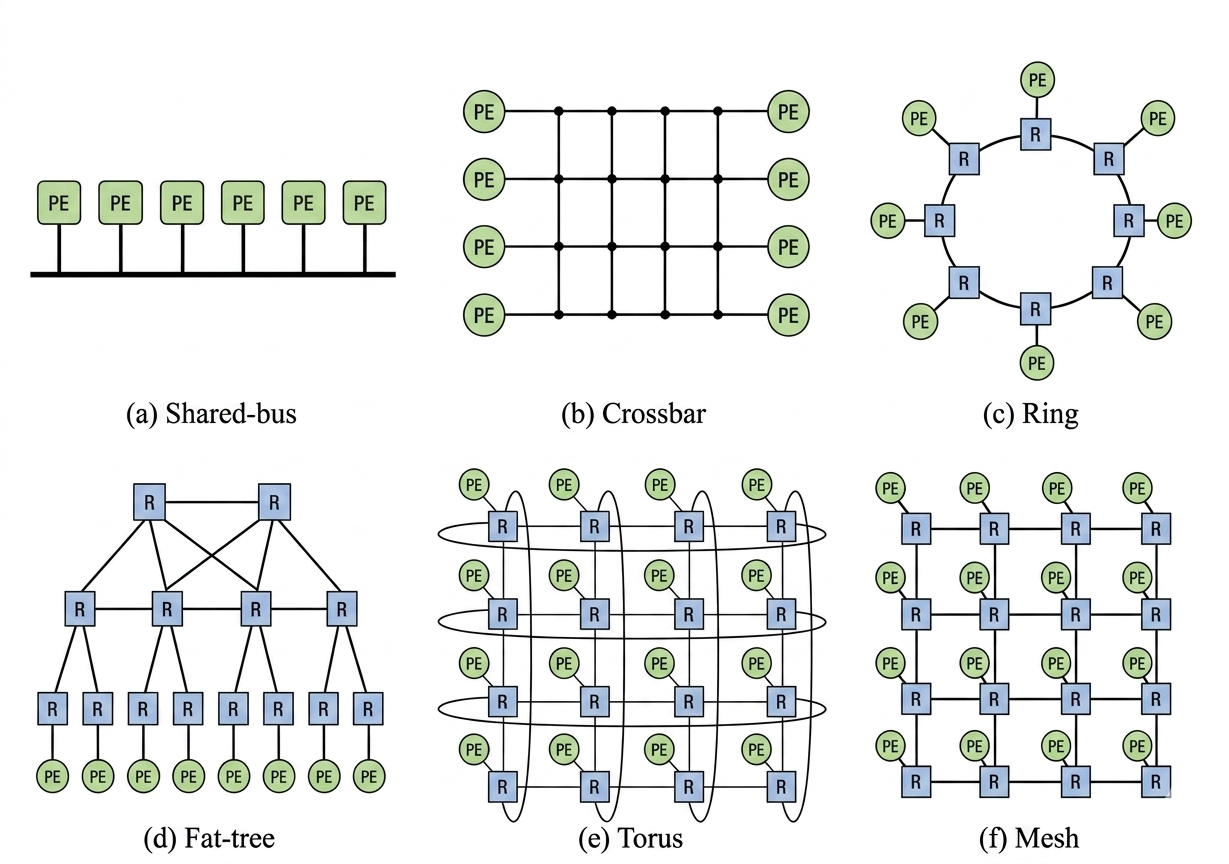
\includegraphics[width=0.8\textwidth]{images/ch2background/network_topology.png}
    \caption{Network topology}
    \label{fig:network_topology}
\end{figure}


\subsection{Flow Control}
Flow control defines how network resources are allocated when data is transmitted from a source node to a destination node through multiple routers and links. Its main purpose is to coordinate the use of communication channels and buffers, especially when multiple packets compete for the same network resource at the same time.

At a high level, two basic switching approaches can be considered: circuit switching and packet switching. In circuit switching, a complete communication path is established before data transmission begins, and the reserved path remains occupied until the transfer is finished. This approach can provide predictable transmission behavior once the connection is set up, but it suffers from long setup time and low channel utilization, since reserved resources may remain idle during parts of the transmission. For this reason, circuit switching is generally not suitable for scalable on-chip communication systems.

In contrast, packet switching does not require a dedicated end-to-end path to be reserved in advance. Instead, a message is divided into smaller transmission units and forwarded hop by hop through the network. This improves resource utilization and allows multiple messages to share the same physical channels. In NoC design, packet switching is more widely adopted because it provides better flexibility and higher throughput under dynamic traffic conditions.

In a packet-switched NoC, data is usually organized hierarchically as message, packet, and flit, as shown in Figure~\ref{fig:packet_flit}. A message is the complete unit of communication between two nodes. A message may be divided into one or more packets, and each packet may be further divided into several flits. The flit is the basic unit handled by the router for flow control. Based on how packets and flits are buffered and forwarded, several packet-switched flow control strategies have been proposed, including store-and-forward, virtual cut-through, and wormhole switching \cite{Danashtalab2014}. These strategies differ mainly in their buffer requirements, latency, and hardware complexity. Among them, wormhole switching is widely used in NoCs because it reduces buffer demand while maintaining relatively efficient packet forwarding. In wormhole switching, a packet is divided into flits, where the head flit carries routing information and establishes the path, the body flits follow the reserved path, and the tail flit releases the occupied resources after the transmission is completed.

\begin{figure}[htbp]
    \centering
    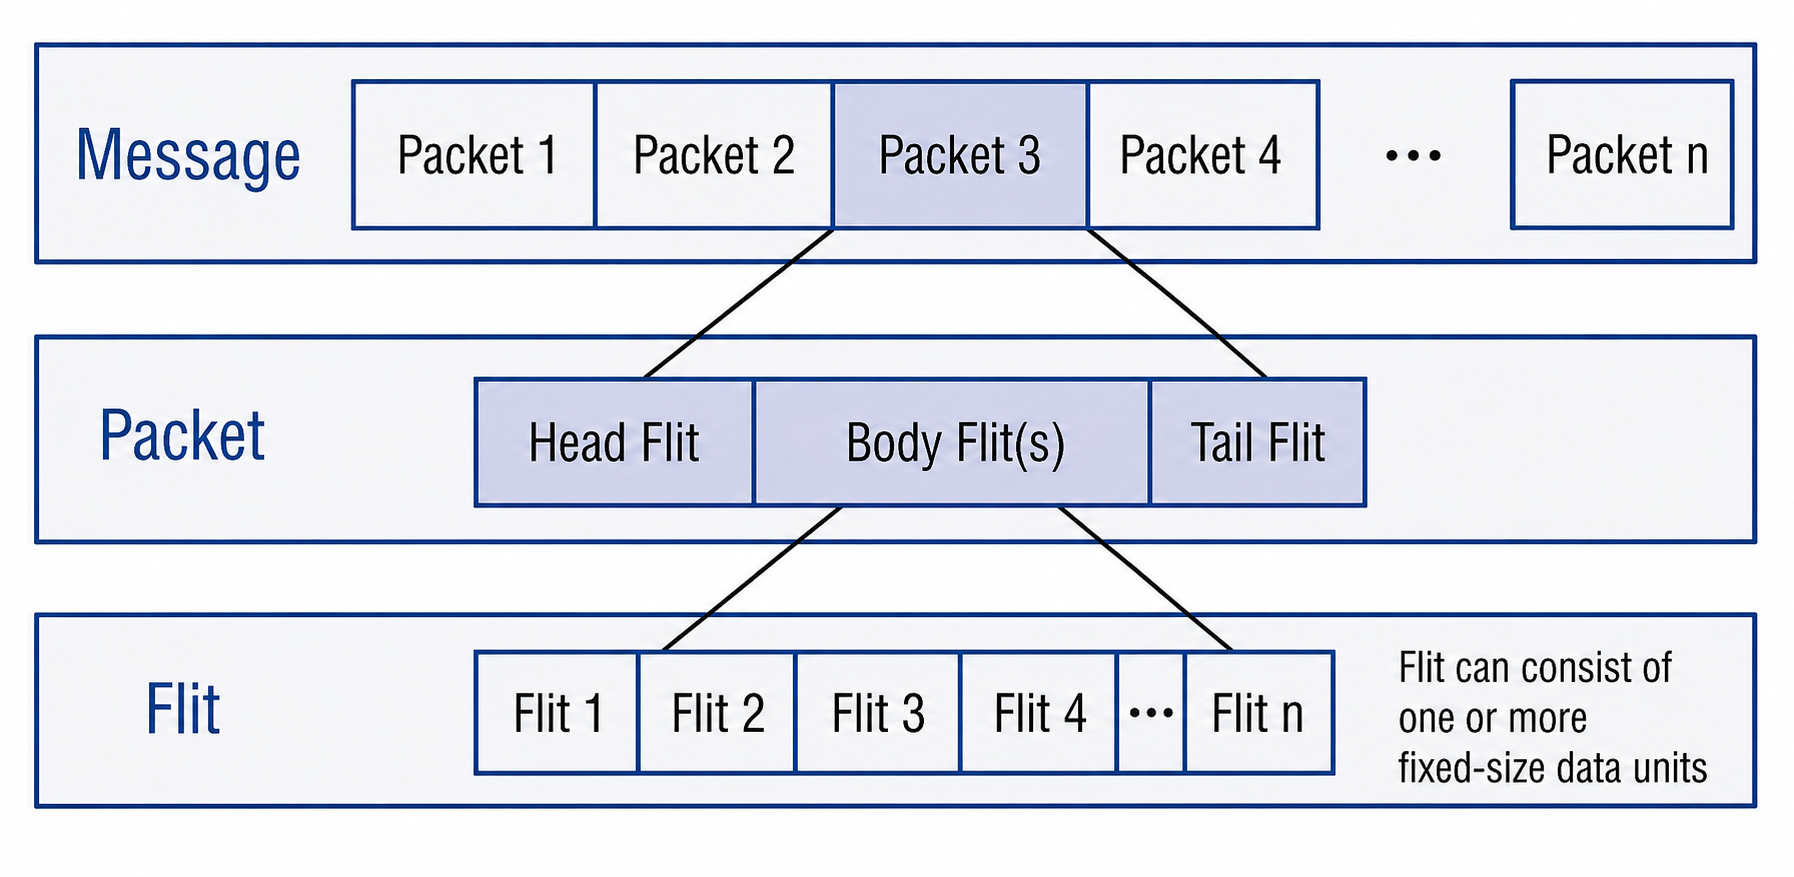
\includegraphics[width=0.8\textwidth]{images/ch2background/packet_flit.png}
    \caption{Packet and flit organization}
    \label{fig:packet_flit}
\end{figure}

Since this thesis focuses on routing and router design in a NoC-based communication structure, packet-switched flow control is adopted, and wormhole switching is used as the main data transmission mechanism.


\subsection{Deadlock}
Deadlock is a critical problem in Network-on-Chip systems, where a group of packets are permanently blocked because each of them is waiting for resources held by others. In packet-switched networks, deadlock usually occurs when packets form a cyclic dependency on channels or buffers, so that none of them can continue to move forward, as shown in Figure~\ref{fig:deadlock}.

\begin{figure}[htbp]
    \centering
    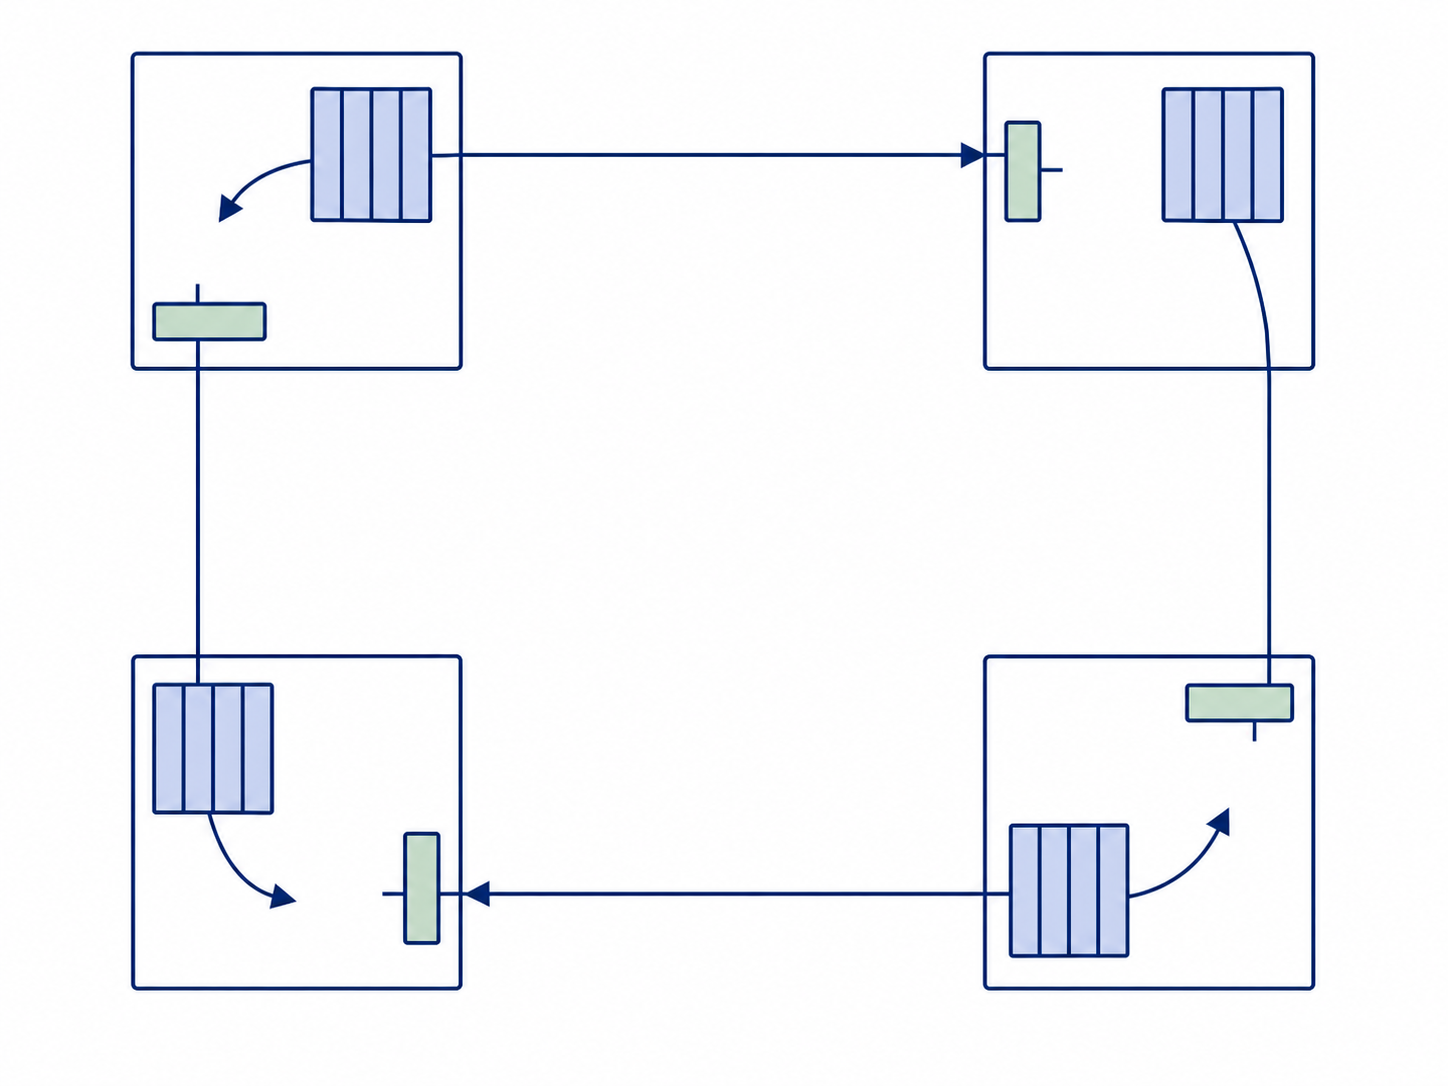
\includegraphics[width=0.6\textwidth]{images/ch2background/deadlock.png}
    \caption{Deadlock scenario caused by cyclic dependency}
    \label{fig:deadlock}
\end{figure}

In wormhole-switched NoCs, deadlock is closely related to buffer occupation and channel allocation. Since packets advance flit by flit and may hold network resources while waiting for the next channel to become available, circular waiting can arise when several packets occupy different resources and simultaneously request one another’s blocked paths. Once such a cycle is formed, the involved packets remain stalled indefinitely unless additional recovery mechanisms are introduced.

Because deadlock can completely stop packet delivery and significantly degrade network reliability, it must be considered carefully in router and routing design. In general, deadlock can be avoided either by designing routing algorithms that eliminate cyclic channel dependencies or by introducing mechanisms such as virtual channels to separate traffic flows and break resource dependency cycles.

\subsection{Virtual Channels}
In wormhole-switched networks, blocking occurs when a packet occupies a physical channel and prevents other packets from using the same path. To alleviate this, virtual channels (VCs) divide one physical channel into multiple logical channels, each with its own buffer and control state. This enables multiple packets to share the same physical link without being forced to wait in a single queue, as illustrated in the Figure~\ref{fig:virtual_channel}, where each input port is equipped with multiple virtual channels.

\begin{figure}[htbp]
    \centering
    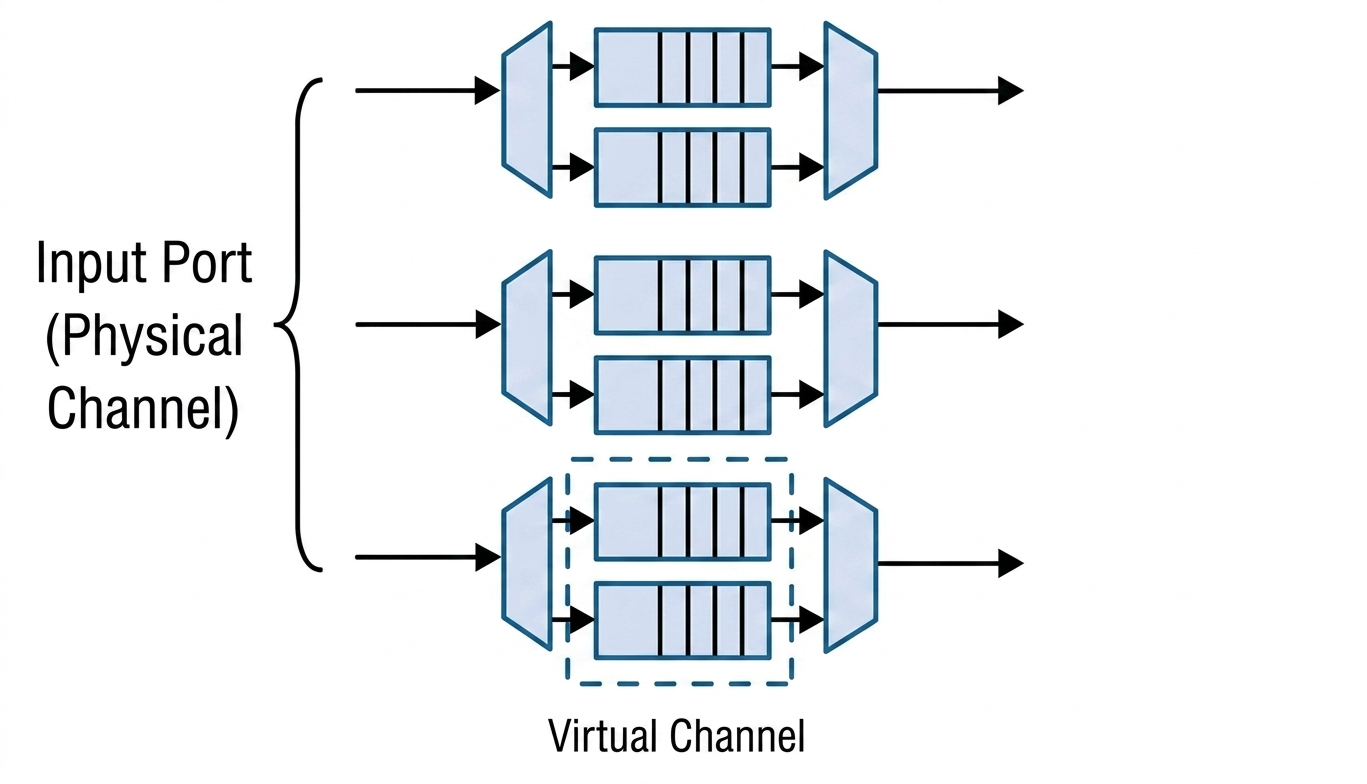
\includegraphics[width=0.6\textwidth]{images/ch2background/virtual_channel.png}
    \caption{Example of three Input Ports with two virtual channels per port}
    \label{fig:virtual_channel}
\end{figure}

At the input side of a router, incoming flits are stored in separate virtual-channel buffers and are later multiplexed onto the output link. If one packet is blocked in a certain virtual channel, packets belonging to other virtual channels may still continue to use the same physical channel. Therefore, virtual channels improve link utilization and reduce the blocking effect caused by resource contention.

Another important benefit of virtual channels is the reduction of head-of-line (HoL) blocking. Without virtual channels, a blocked packet at the front of a queue may prevent all following packets from moving forward, even if their desired paths are available. By separating packets into different virtual channels, this unnecessary blocking can be reduced, which improves overall network throughput and latency.

Virtual channels are also commonly used to support deadlock avoidance in NoC design. By assigning packets to different channel classes, cyclic resource dependencies can be reduced or eliminated. However, these benefits come at the cost of additional buffers, control logic, and allocation complexity in the router design.

\subsection{Router Microarchitecture}
The router is the key component of a Network-on-Chip, since it determines how flits are buffered, arbitrated, and forwarded between input and output ports. In a typical NoC router, each arriving flit first enters an input buffer, where it waits until the required output resource becomes available. Compared with traditional large-scale network routers, NoC routers are designed under much stricter latency, area, and power constraints. Therefore, their microarchitecture must provide efficient packet forwarding while keeping implementation complexity low.

The main task of the router is to transfer each incoming flit from the selected input virtual channel to the appropriate output port. To achieve this, several functions must be completed inside the router. First, the router determines the desired output direction according to the routing algorithm. For head flits, this step also identifies the candidate output virtual channels. Next, a virtual-channel allocation stage assigns an available output virtual channel to the packet. After that, switch allocation is performed to resolve contention among multiple input flits requesting the same output port. Once the allocation is granted, the flit traverses the internal crossbar and is forwarded to the output side of the router.

Figure~\ref{fig:router} shows the virtual-channel-based router architecture.

\begin{figure}[htbp]
    \centering
    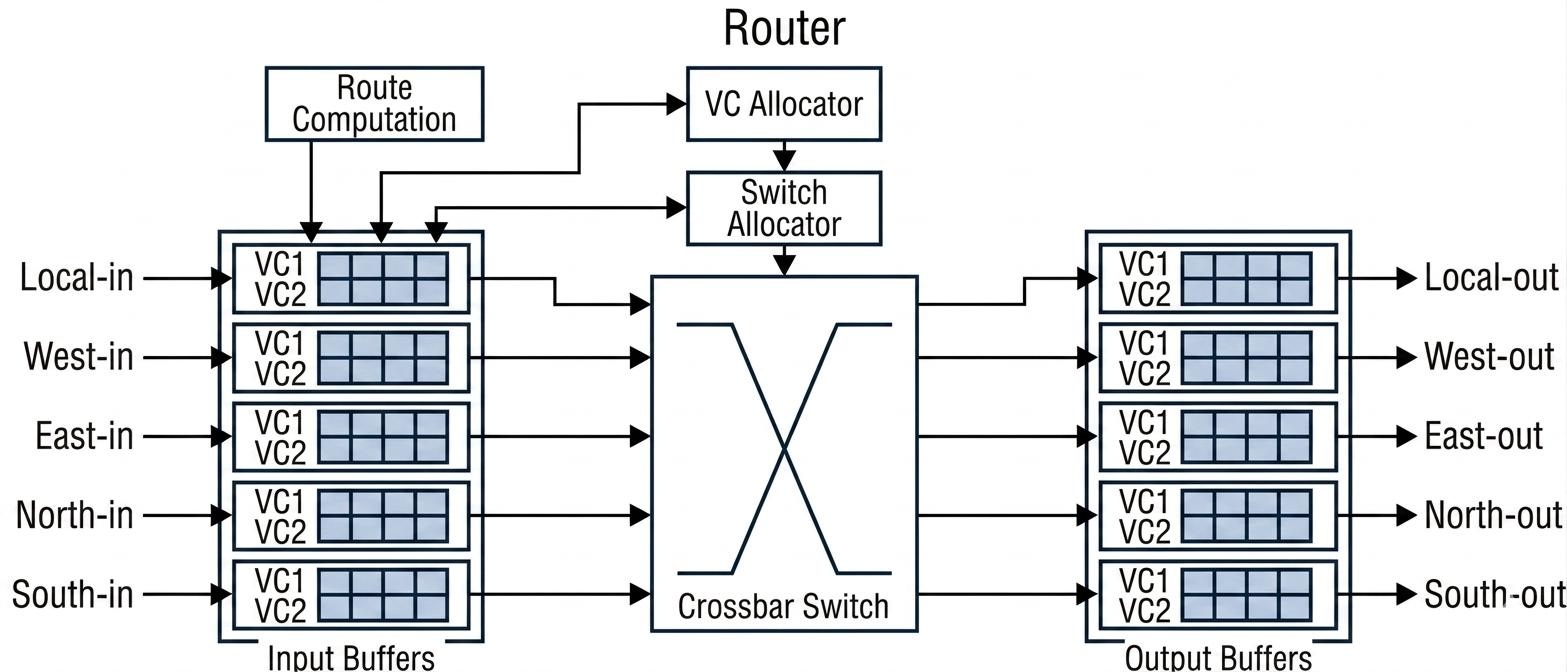
\includegraphics[width=0.85\textwidth]{images/ch2background/router.png}
    \caption{Virtual-channel-based router architecture}
    \label{fig:router}
\end{figure}

\begin{itemize}
    \item \textbf{Input buffers:}

    Input buffers temporarily store incoming flits before they are forwarded. They provide waiting space when the requested output resource is not immediately available.

    \item \textbf{Routing computation:}

    The routing computation logic determines the output port for an incoming packet according to the selected routing algorithm.

    \item \textbf{Virtual-channel allocator:}

    The virtual-channel allocator assigns an available output virtual channel to a packet, usually based on the routing result and channel availability.

    \item \textbf{Switch allocator:}

    The switch allocator resolves contention among multiple input flits requesting the same output port and decides which flit can access the crossbar in the current cycle.

    \item \textbf{Crossbar switch:}

    The crossbar switch provides the internal data path between input ports and output ports, allowing the selected flit to be transferred to its destination output.
\end{itemize}

To improve operating frequency, router operation is usually organized as a pipeline. A common pipelined flow includes buffer write, route computation, virtual-channel allocation, switch allocation and switch traversal. For body and tail flits, route computation and virtual-channel allocation are usually not repeated, since they inherit the routing and channel information established by the head flit. This reduces control overhead and improves forwarding efficiency.

Overall, router microarchitecture has a direct impact on network latency, throughput, area, and power consumption. Efficient design of buffers, allocators, and crossbar organization is therefore essential for building a practical NoC communication system.


\chapter{Design and Implementation}
\label{ch3:design_and_implementation}

\section{Design Targets}
The objective of this work is to design and implement a Network-on-Chip (NoC) router for a $3 \times 3$ mesh system. The target mesh structure is illustrated in Figure~\ref{fig:mesh_3x3_pe}. The router is designed to support packet-based communication using fixed-width flits and deterministic XY routing, while also providing virtual-channel-based flow control.

\begin{figure}[htbp]
    \centering
    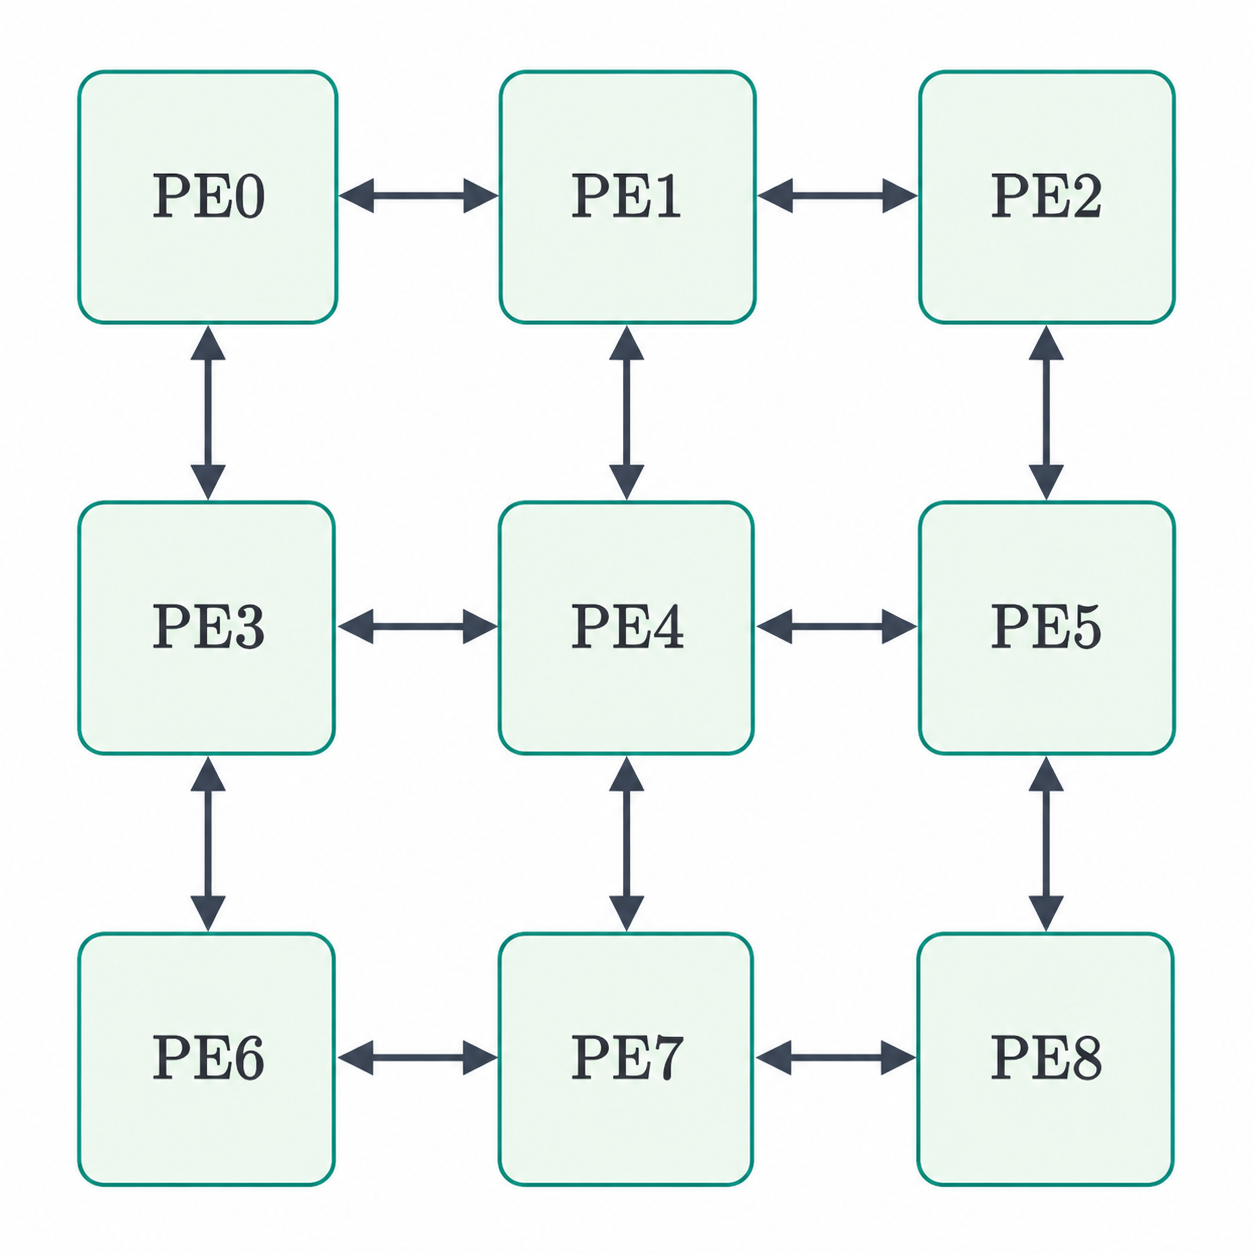
\includegraphics[width=0.4\textwidth]{images/ch3_design_and_implementation/3_times_3_mesh.png}
    \caption{$3 \times 3$ mesh structure}
    \label{fig:mesh_3x3_pe}
\end{figure}

The router first needs to provide the basic packet forwarding function. Each packet is sent from a source processing element to a destination processing element, and the routing decision is made according to the information carried in the header flit. Since a packet is divided into several flits, the router also has to make sure that flits belonging to the same packet follow the same reserved path and keep their original order. 

To organize the router operation, a three-stage pipeline is used. The first stage performs routing computation and virtual-channel allocation. The second stage is responsible for switch allocation, where the router decides which input can access the requested output port. The third stage performs switch traversal and sends the selected flit to the output side. By separating these functions into different stages, the design avoids putting too much logic into a single cycle and makes the implementation easier to meet timing.

Flow control is another important requirement in the router design. Since downstream buffers may become full, the router must be able to stop sending flits when the next router cannot accept more data. For this reason, the interface uses a valid-ready handshake together with credit-based flow control. A flit is transferred only when both valid and ready are asserted, while the returned credit information is used to indicate available buffer space in the downstream virtual channels.

Overall, the goal of this chapter is to present not only the implemented router structure, but also the design method used to connect routing decisions, virtual-channel allocation, flow control, and hardware implementation in a consistent router architecture.
\section{Router Architecture}
The design is based on a $3 \times 3$ two-dimensional mesh topology, in which nine processing elements are interconnected by routers. Each router contains five ports: one local port connected to the processing element, and four directional ports connected to the north, south, west, and east neighbors. This topology provides the communication framework for packet transmission in the target system.

Figure~\ref{fig:router_microarchitecture} illustrates the overall architecture of the proposed router. The router is designed to support flit-based packet forwarding under wormhole switching and virtual-channel flow control. In general, the router consists of routing computation, virtual-channel allocation, switch allocation, and switching logic, together with the required state management units. These modules cooperate to determine the output direction, assign channel resources, and transfer flits from the selected input side to the corresponding output side.The following sections describe the structure and implementation of these modules in more detail.

\begin{figure}[htbp]
    \centering
    \includegraphics[width=0.9\textwidth]{images/ch3_design_and_implementation/router_microarchitec.png}
    \caption{Router microarchitecture}
    \label{fig:router_microarchitecture}
\end{figure}

\section{Parameter Definition}
The main configuration parameters of the proposed router are summarized as follows:

\begin{itemize}
    \item \textbf{Topology and Node Definition:}

    The design is based on a $3 \times 3$ two-dimensional mesh topology, in which nine processing elements communicate through interconnected routers. Each router is identified by its Cartesian coordinates (x,y), where each coordinate ranges from 0 to 2. This coordinate-based representation provides a direct way to identify the position of each node in the network. 

    \item \textbf{Port Configuration:}

    Each router contains five ports, including one local port connected to the processing element and four directional ports connected to the north, south, west, and east neighboring routers. This five-port organization defines the communication interface of the router in the target mesh network. 
\[
\texttt{port\_t} \in \{\texttt{LOCAL}, \texttt{NORTH}, \texttt{SOUTH}, \texttt{WEST}, \texttt{EAST}\}.
\]
    \item \textbf{Packet and Flit Configuration:}

    For data transmission, packets are divided into 32-bit flits. The supported flit types include head flits, body flits, tail flits, and head-tail flits. Among them, the head flit carries the control and routing information required for packet forwarding. This information is organized into several header fields, including source and destination coordinates, flit type, packet length, virtual-channel information, and message-related fields. The header format and the detailed field definitions are shown in Figure~\ref{fig:header_format} and Table~\ref{tab:header_flit_fields}, respectively.
\[
\texttt{flit\_type\_t} \in \{\texttt{FLIT\_HEAD}, \texttt{FLIT\_BODY}, \texttt{FLIT\_TAIL}, \texttt{FLIT\_HEADTAIL}\}.
\]

\begin{figure}[htbp]
    \centering
    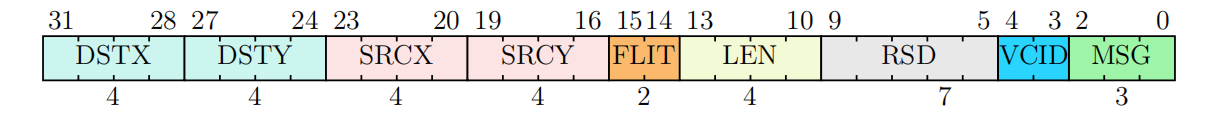
\includegraphics[width=0.8\textwidth]{images/ch3_design_and_implementation/header_flit_field.png}
    \caption{Header flit format and field definitions}
    \label{fig:header_format}
\end{figure}

\begin{table}[htbp]
    \centering
    \caption{Header Flit Fields}
    \label{tab:header_flit_fields}
    \begin{tabular}{llll}
        \hline
        \textbf{Field Name} & \textbf{Bit Slice} & \textbf{Width} & \textbf{Description} \\
        \hline
        DSTX & [31:28] & 4 & Destination ID. \\
        DSTY & [27:24] & 4 & Destination ID. \\
        SRCX & [23:20] & 4 & Source ID. \\
        SRCY & [19:16] & 4 & Source ID. \\
        FLIT & [15:14] & 2 & Flit Type. \\
        LEN  & [13:10] & 4 & Packet Length. \\
        VCID & [4:3]   & 2 & Next Hop IVC ID. \\
        MSG  & [2:0]   & 3 & Message Class. \\
        \hline
    \end{tabular}
\end{table}

    \item \textbf{Virtual Channel Configuration:}

    To support virtual-channel flow control, each router contains five ports, and each port is associated with both input-side and output-side virtual channels. Specifically, each input port contains four input virtual channels (IVCs), and each output port contains four output virtual channels (OVCs). Therefore, one router includes a total of 20 input virtual channels and 20 output virtual channels. These virtual channels provide the buffering and allocation resources required for flit storage, channel assignment, and packet forwarding in the router design.
\end{itemize}

\section{Handshake and Credit-based Flow Control}
The router adopts a two-way flow-control mechanism that combines a forward valid-ready handshake with backward credit return. The forward path transfers the flit data and its associated control information, while the backward path reports buffer-release events from the downstream router through \texttt{credit\_return}. Together, these mechanisms determine when a flit can safely move to the next router. This flow-control mechanism is illustrated in Fig.~\ref{fig:handshake_and_credit-based_flow_control}.

\begin{figure}[htbp]
    \centering
    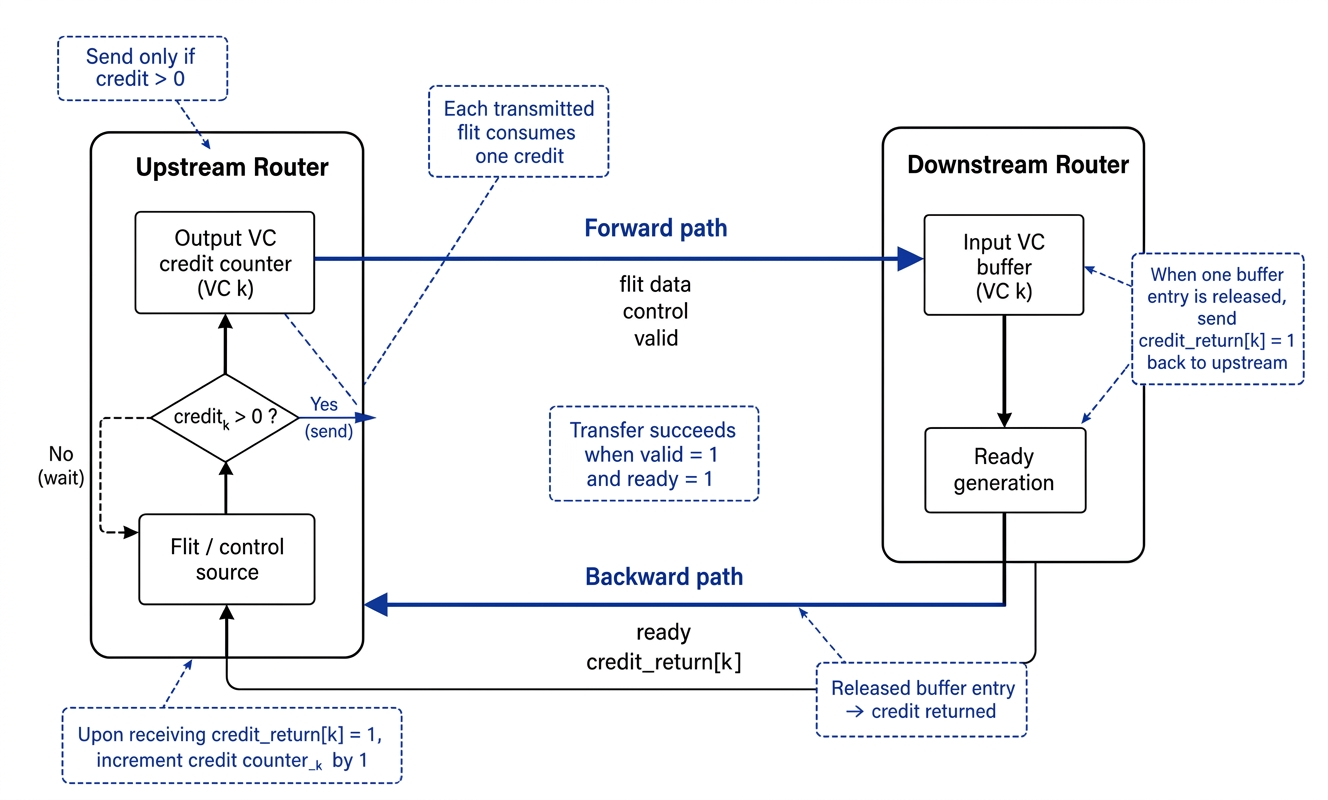
\includegraphics[width=0.85\textwidth]{images/ch3_design_and_implementation/handshake.png}
    \caption{Valid-ready handshake and credit-based flow control between neighboring routers.}
    \label{fig:handshake_and_credit-based_flow_control}
\end{figure}

In the forward path, a flit transfer is completed only when \texttt{valid} and \texttt{ready} are both asserted in the same clock cycle. The \texttt{valid} signal is generated by the sender to indicate that the current flit and its control fields are available, while \texttt{ready} is generated by the receiver to indicate that it can accept the flit in the current cycle. If \texttt{valid} is high but \texttt{ready} is low, the sender keeps the current flit and control signals stable until the handshake succeeds.

The credit return path is used to track the availability of downstream virtual-channel buffers. When \texttt{credit\_return[k] = 1}, one buffer entry in downstream input virtual channel \texttt{k} has been released. The upstream router then increments the corresponding output virtual-channel credit counter. Before scheduling a flit to an output virtual channel, the router checks whether the corresponding credit count is non-zero. A flit can be selected for transmission only when downstream buffer space is available, and each successful advancement consumes one credit.

In this design, the valid-ready handshake controls whether a flit is transferred in the current cycle, while the credit mechanism tracks downstream buffer availability across cycles. By combining these two mechanisms, the router avoids downstream buffer overflow and propagates backpressure when congestion occurs. This provides controlled and reliable flow-control behavior for pipelined flit transmission.

\section{Routing Algorithm}
The router uses a deterministic XY routing algorithm in the 3×3 mesh network. The output port is selected by comparing the current router coordinates with the destination coordinates in the header flit.

The packet is first routed in the X direction. If the destination is on the right, the packet is sent to EAST; if it is on the left, it is sent to WEST. When the X coordinate is already matched, the router then compares the Y coordinate and sends the packet to NORTH or SOUTH. If both coordinates match, the packet is delivered to the LOCAL port.

This method is simple and hardware-efficient, since it only requires coordinate comparison and no routing table. Another advantage is that XY routing naturally restricts all turns from the Y dimension back to the X dimension. Therefore, cyclic channel dependencies are avoided, which helps prevent routing deadlock. Its limitation is that the path is fixed and cannot adapt to congestion.

\begin{algorithm}[htbp]
\caption{Pseudo code of the XY-routing computation}
\label{alg:xy_routing}
\textbf{Definitions:}

\begin{itemize}
    \item $cur_x, cur_y$: current router coordinates.
    \item $dst_x, dst_y$: destination router coordinates.
    \item $port$: selected output port.
\end{itemize}

\textbf{Input:}

\begin{itemize}
    \item $cur_x, cur_y$: coordinates of current router.
    \item $dst_x, dst_y$: coordinates extracted from the header flit.
\end{itemize}

\textbf{Output:}

\begin{itemize}
    \item $port$: routing decision toward the next hop.
\end{itemize}

\begin{algorithmic}[1]
\If{$dst_x > cur_x$}
    \State $port \gets EAST$
\ElsIf{$dst_x < cur_x$}
    \State $port \gets WEST$
\ElsIf{$dst_y > cur_y$}
    \State $port \gets NORTH$
\ElsIf{$dst_y < cur_y$}
    \State $port \gets SOUTH$
\Else
    \State $port \gets LOCAL$
\EndIf
\State \Return $port$
\end{algorithmic}
\end{algorithm}


\section{Allocators and Arbiters}
In a NoC router, multiple flits may request the same limited resource in the same cycle. For example, several input virtual channels may request the same output virtual channel, or several input ports may try to access the same output port of the switch. Since each resource can only be used by one flit or packet at a time, arbitration is required to decide which request should be served.

An arbiter is used when multiple requesters compete for one shared resource. It receives several request signals and grants the resource to one selected requester. In contrast, an allocator handles a more general case where multiple requesters compete for multiple resources. Therefore, an allocator can be viewed as a structure built from several arbiters to generate a conflict-free matching between requesters and resources.

In this router, allocation is mainly used in two places. The first one is virtual-channel allocation, where input virtual channels compete for available output virtual channels. The second one is switch allocation, where flits from different input sides compete for access to output ports through the switch. Since these allocation steps are on the critical path of router operation, the allocator should be simple, fast, and suitable for hardware implementation. Therefore, this design uses a separable input-first allocation method based on round-robin arbiters.

\subsection{Round-robin Arbiter}
A round-robin arbiter is used as the basic arbitration unit in the allocator. The basic structure of the round-robin arbiter is shown in Figure~\ref{fig:rr_arbiter}. The round-robin arbiter used in this design is implemented using a rotating priority pointer and fixed-priority arbitration. The pointer \texttt{ptr} indicates the requester with the highest priority in the current arbitration round. Based on this pointer, the request vector is divided into a masked region and a wrap-around region. The masked request vector is first processed by a fixed-priority arbiter. If no active request exists in the masked region, the original unmasked request vector is arbitrated instead to complete the wrap-around selection.

\begin{figure}[htbp]
    \centering
    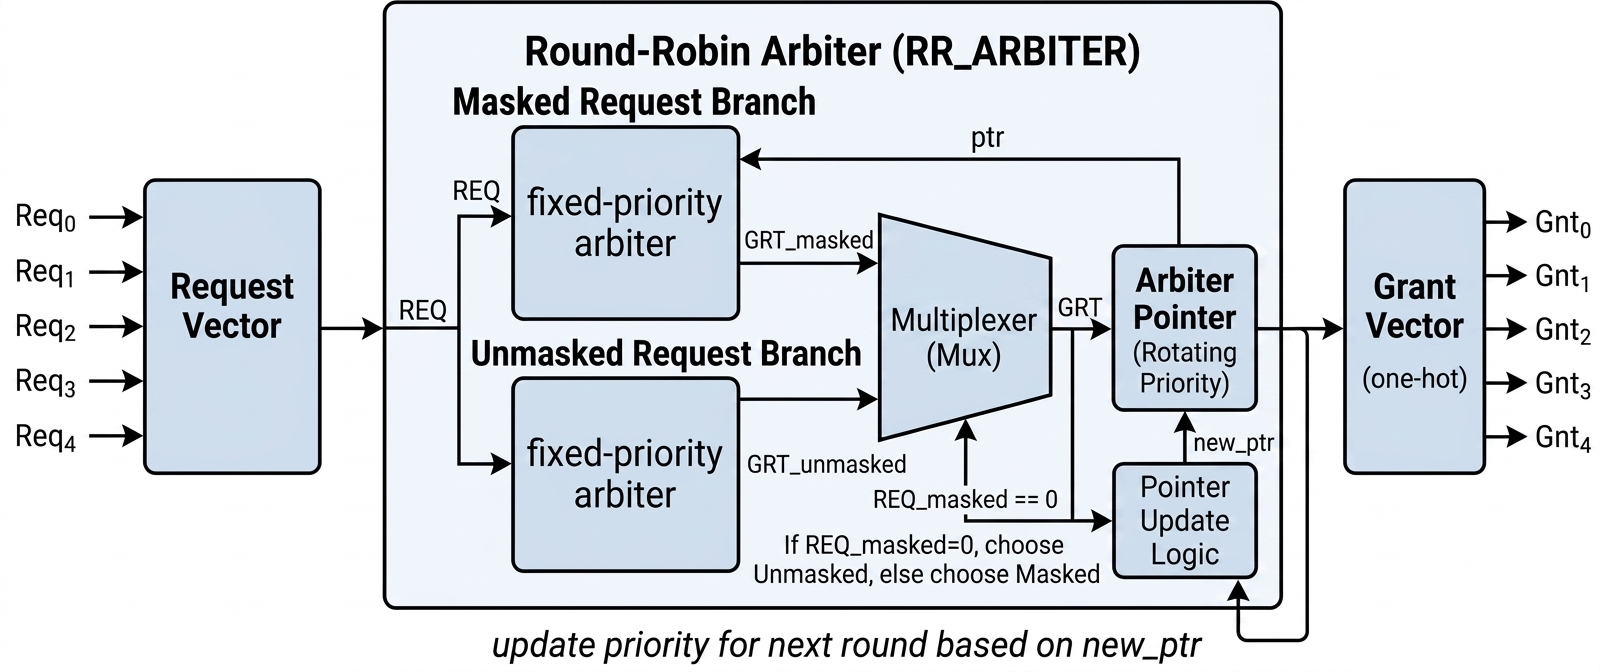
\includegraphics[width=0.85\textwidth]{images/ch3_design_and_implementation/round_robin_arbiter.png}
    \caption{Round-robin arbiter structure}
    \label{fig:rr_arbiter}
\end{figure}

After a grant is generated, the pointer is updated to the requester immediately following the granted one. Therefore, the winning requester is moved to the lowest priority position in the next arbitration round. When arbitration is not enabled or no request is active, the pointer remains unchanged. Compared with a fixed-priority arbiter, this rotating-priority mechanism provides better fairness, prevents one requester from continuously occupying the shared resource, and reduces the possibility of starvation.

\subsection{Separable Input-first Allocation}
A separable allocator is used to handle the case where multiple requesters compete for multiple resources. Instead of performing one large global arbitration, the allocation problem is divided into two simpler arbitration steps. This reduces hardware complexity and makes the allocator easier to pipeline and implement in RTL.

The allocator uses a separable input-first allocation strategy. The requesters are first grouped by input side. In the first arbitration step, each input side selects at most one candidate request from all its active requests. This means that one input can only forward one request to the second arbitration step in a given cycle. In the second step, each resource arbitrates among the candidate requests that target it and selects one final winner.

The overall organization of the separable input-first allocator is shown in Figure~\ref{fig:separable_input_first_allocation}. In this router, the separable input-first allocator operates on the requests from the virtual channels of five input ports. In the first level, each input-side arbiter selects at most one requesting virtual channel from the local VCs of the same input port. This produces one candidate request per input port. In the second level, the selected candidates are grouped according to their target output ports. Each output-side arbiter then selects one winning input among the candidates requesting the same output port. Since the router has five output ports, this stage ensures that each output port accepts at most one input in one cycle. Finally, the selected winners are mapped back to the original virtual channels to generate the final grant signals. In this way, the allocator guarantees that each input port grants at most one VC and each output port is assigned to at most one input.

\begin{figure}[htbp]
    \centering
    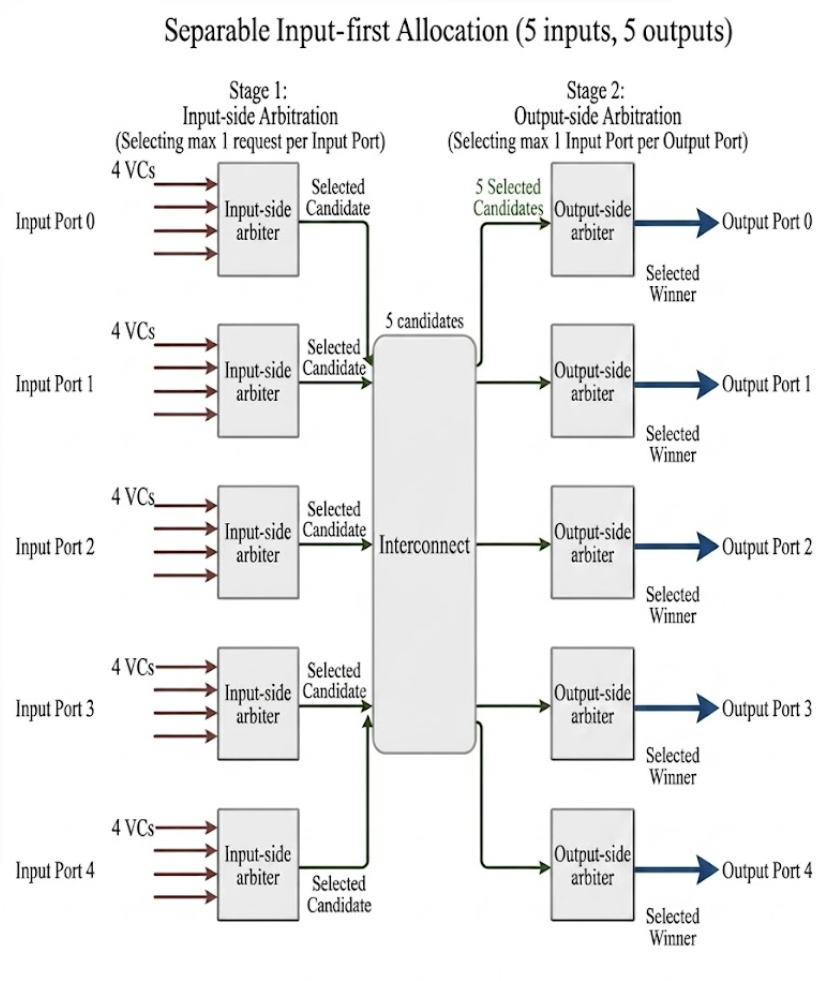
\includegraphics[width=0.8\textwidth]{images/ch3_design_and_implementation/Separable_Input_first_Allocation.png}
    \caption{Separable input-first allocation structure}
    \label{fig:separable_input_first_allocation}
\end{figure}

Figure~\ref{fig:separable_input_first_example} illustrates an example of separable input-first allocation with five inputs and five output resources. In Figure~\ref{fig:separable_input_first_example}(a), the request matrix shows all active requests before arbitration. After the first-stage input-side arbitration, each input keeps at most one selected request, forming the intermediate matrix shown in Figure~\ref{fig:separable_input_first_example}(b). The second-stage output-side arbitration then resolves conflicts among requests targeting the same output resource, and the final grant matrix is shown in Figure~\ref{fig:separable_input_first_example}(c). The final grant matrix contains only conflict-free grants, where each input receives at most one resource and each resource is assigned to at most one input.

\begin{figure}[htbp]
    \centering
    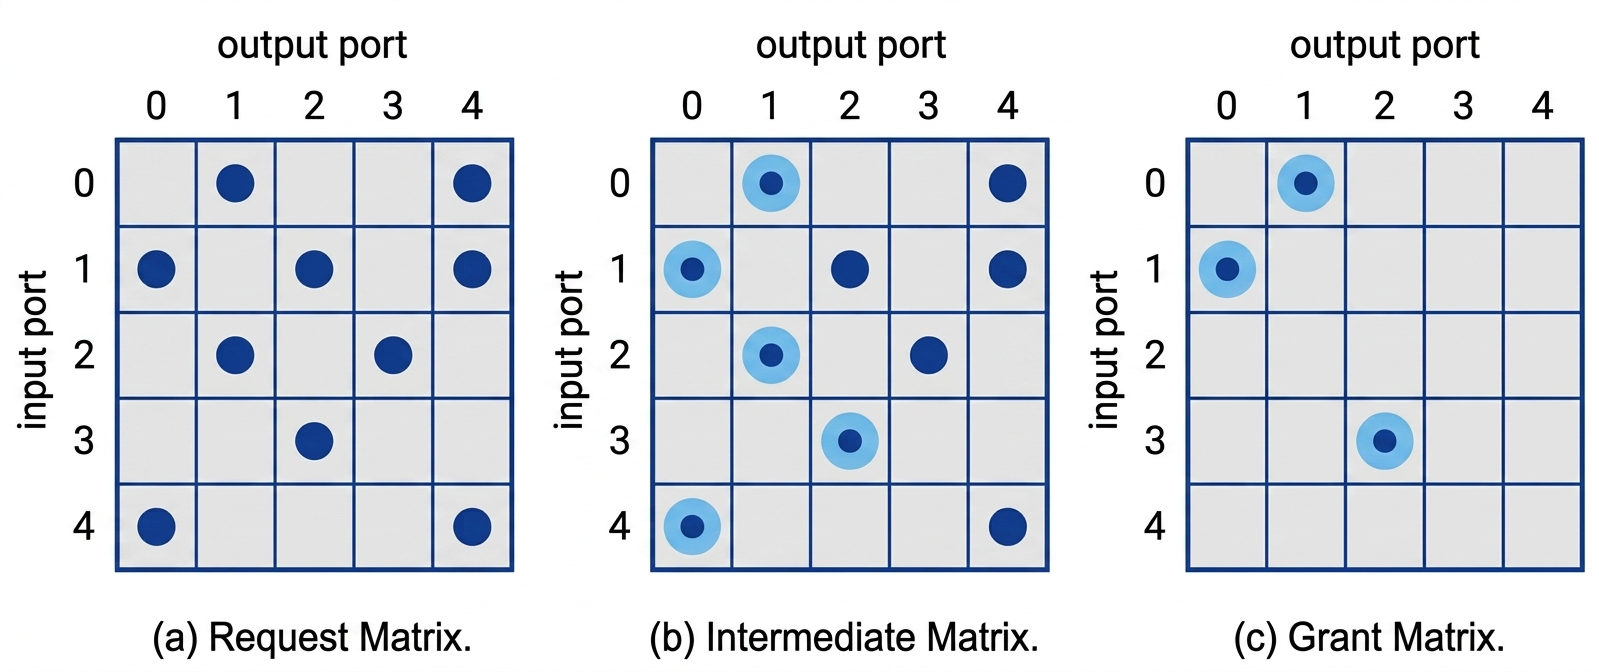
\includegraphics[width=0.9\textwidth]{images/ch3_design_and_implementation/matrix.png}
    \caption{Example of separable input-first allocation.}
    \label{fig:separable_input_first_example}
\end{figure}

The allocation result must still satisfy the basic matching rules: one requester can receive at most one grant, and one resource can be granted to at most one requester. Therefore, the final output of the allocator is a conflict-free grant result.

This approach is suitable for the router design because both virtual-channel allocation and switch allocation involve many requesters and multiple possible resources. By decomposing the allocation into two stages, the design avoids a large centralized allocator and keeps the arbitration logic relatively simple. The drawback is that separable input-first allocation may not always generate the maximum possible number of grants, because the first-stage arbiters make local decisions without knowing the final result of the second stage. However, this trade-off is acceptable for this design, since the main goal is to keep the router simple, predictable, and hardware-efficient.
\subsection{Virtual Channel Allocation}
The virtual-channel allocator is responsible for assigning an available output virtual channel to an input virtual channel. VC allocation is only performed for head flits. When the front flit of an input VC is a head flit, the allocator uses the routing result to identify the requested output port and checks the available output VCs at that port. The availability information is then combined with the candidate VC set to form the final set of allocatable output VCs.

If at least one valid candidate output VC exists, the corresponding input VC sends a request to the separable input-first allocator. The separable allocator then resolves competition among input VCs and output resources using the two-stage arbitration method described previously. When an input VC wins the allocation, the VC allocator generates a grant signal and a one-hot selected output VC signal for that input VC.

After a successful allocation, an update signal is sent to the state unit to mark the selected output VC as occupied. In this way, the VC allocation process can be summarized as three steps: candidate filtering, separable input-first arbitration, and output VC state update. Figure~\ref{fig:vc_allocation_flow} provides an overview of this allocation flow and the relationship among these three stages.

\begin{figure}[htbp]
    \centering
    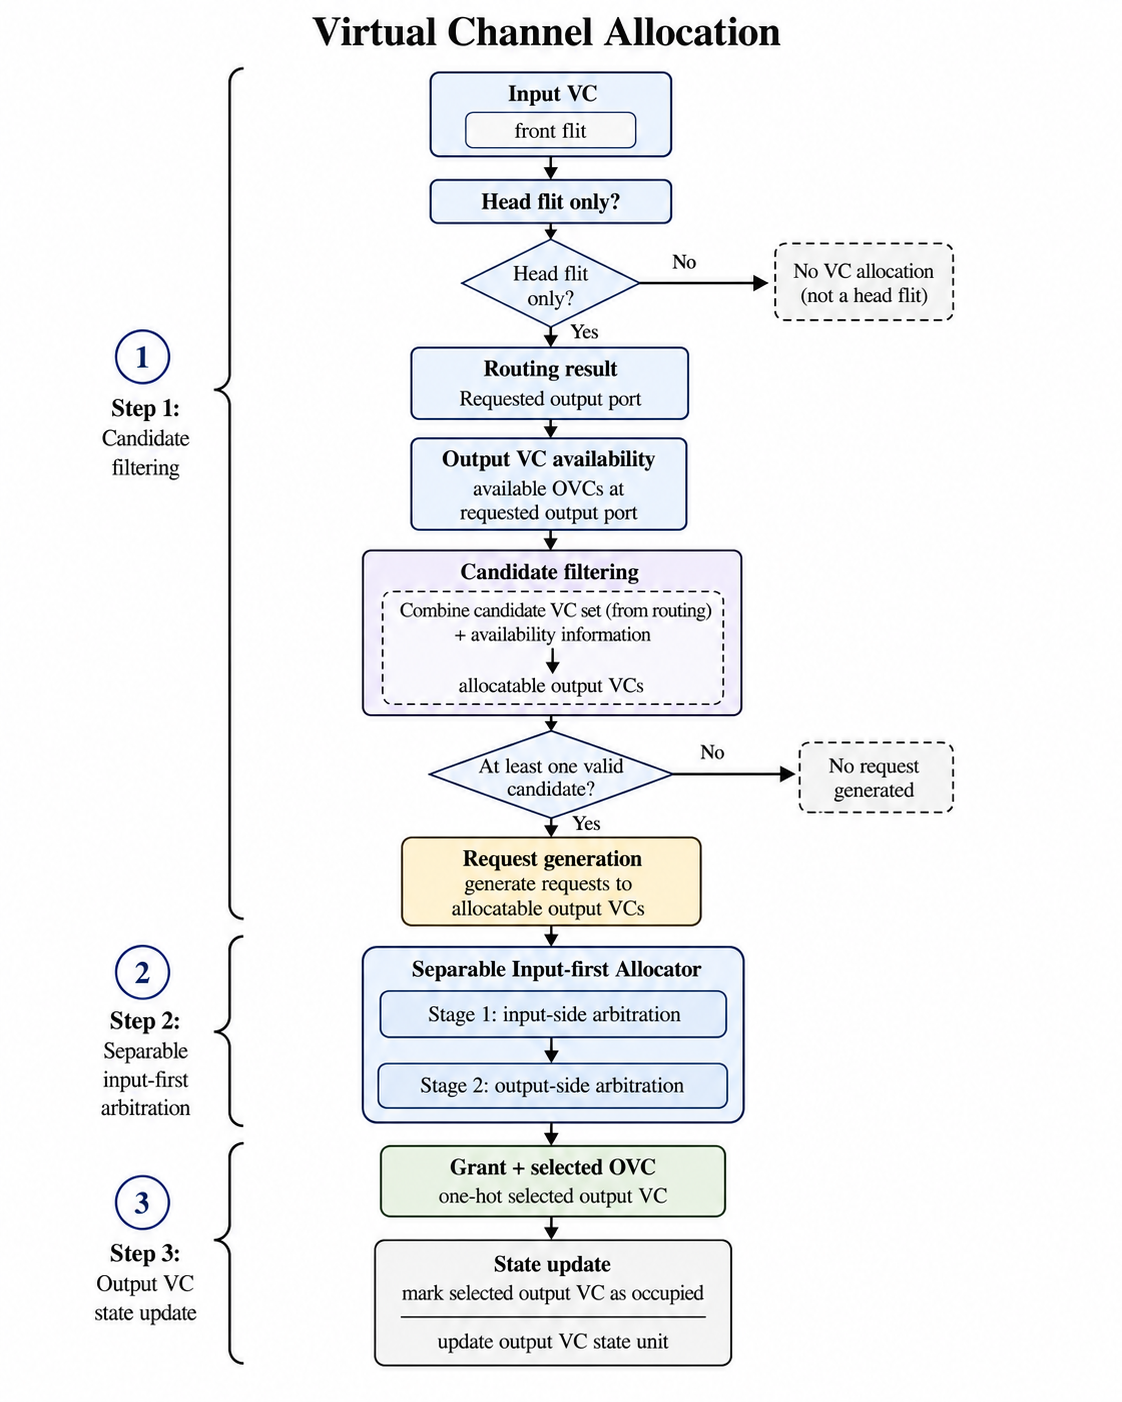
\includegraphics[width=0.8\textwidth]{images/ch3_design_and_implementation/virtual_channel_allocation.png}
    \caption{Virtual-channel allocation flow}
    \label{fig:vc_allocation_flow}
\end{figure}

\subsection{Switch Allocation}
After virtual-channel allocation assigns an output port and an output virtual channel to a packet, each flit of the packet still needs to obtain permission to traverse the router switch. This permission is determined by the switch allocator. In each cycle, the switch allocator selects the input flits that are allowed to access the crossbar and generates the corresponding switch control signals.

The switch allocation process follows the same separable input-first idea introduced earlier. Each input port first arbitrates among its local virtual channels and selects at most one flit that is ready to move forward. As a result, only one request from each input port can be sent to the output side in a cycle. The selected requests are then grouped according to their target output ports. If several input ports request the same output port, the output-side arbiter grants only one of them. The winning input-output pair is then used to configure the crossbar traversal path for that cycle. Figure~\ref{fig:switch_allocation_flow} summarizes the overall switch allocation procedure.

Credit availability is also considered before a flit is allowed to participate in switch allocation. A flit is considered ready only if its assigned downstream virtual channel has available buffer space. When a flit is successfully selected and moves forward, the corresponding credit is consumed. Therefore, switch allocation is not only responsible for crossbar scheduling, but also works together with credit-based flow control to avoid sending flits into a full downstream buffer.

Overall, switch allocation determines the cycle-by-cycle movement of flits through the router. It ensures that each input port sends at most one flit and each output port receives at most one flit in a cycle, while maintaining correct backpressure behavior through credit checking.

\begin{figure}[htbp]
    \centering
    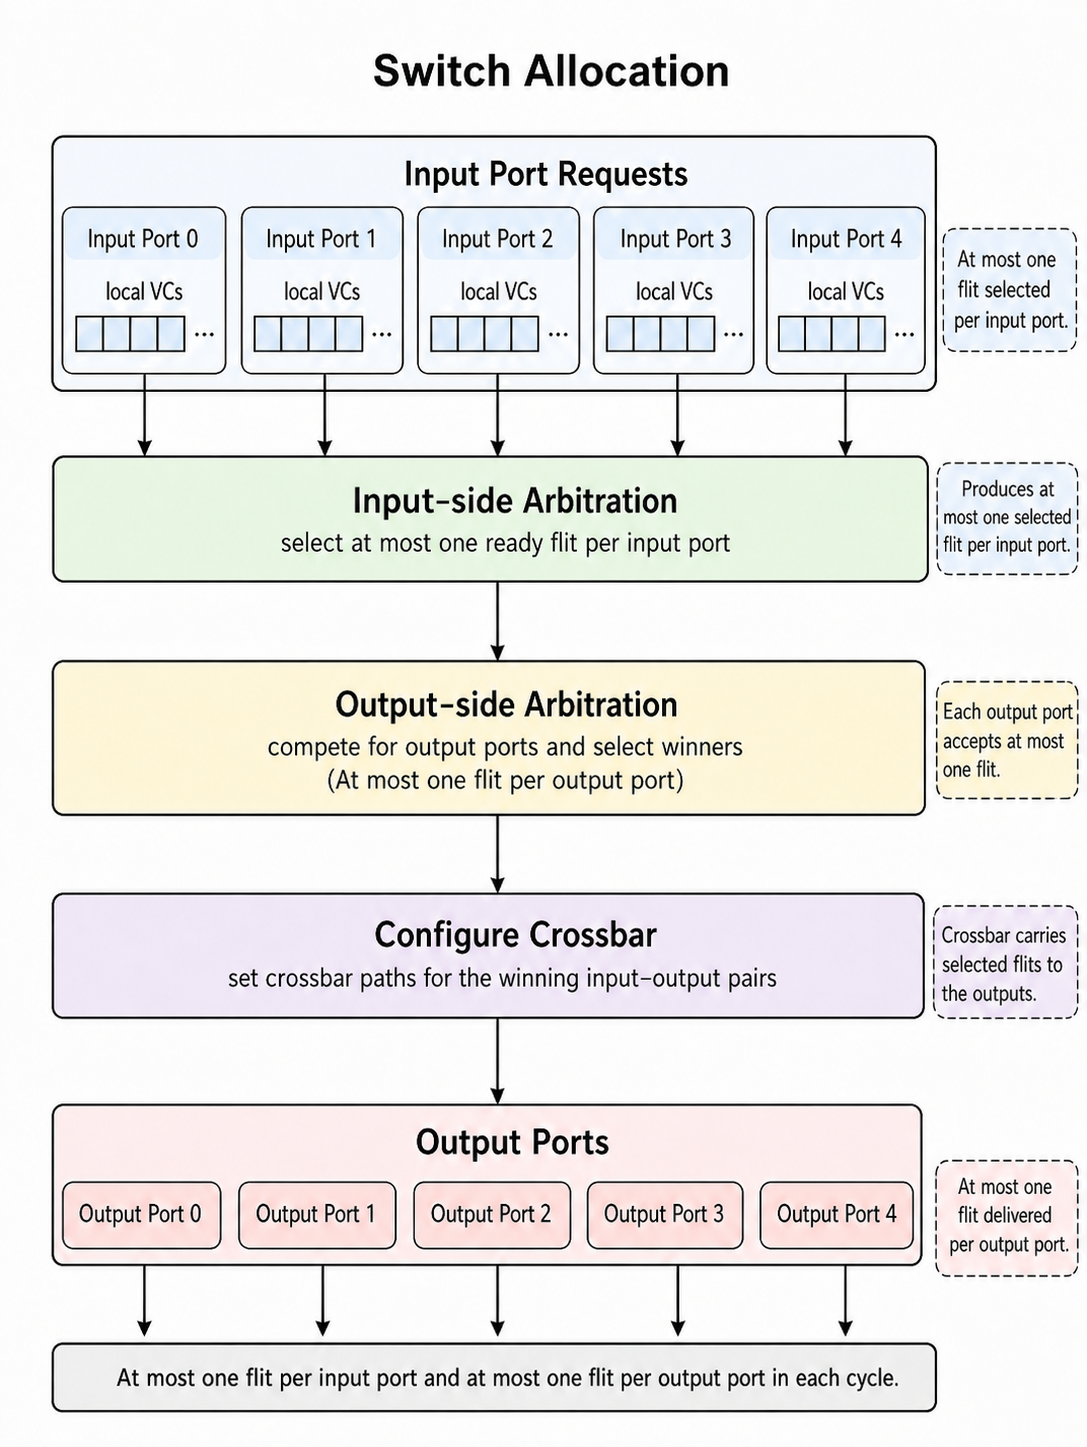
\includegraphics[width=0.6\textwidth]{images/ch3_design_and_implementation/switch_allocation.png}
    \caption{Switch allocation flow}
    \label{fig:switch_allocation_flow}
\end{figure}


\section{Pipeline Organization}

\subsection{Stage 1: Routing Computation and Virtual-channel Allocation}
In the first stage, the router inspects the front flit of each input virtual-channel FIFO. The front flit can be checked without being immediately removed from the buffer. If the front flit is a head flit and the corresponding input VC is not already locked by a previous packet, the router decodes the destination information from the header and performs XY routing to determine the requested output port.

After the output port is determined, the router tries to allocate an available output virtual channel at that port. If the allocation succeeds, the selected output port and output VC are stored in the first-stage pipeline registers. At the same time, an input-VC lock is established. This lock records the reserved output port and output VC, so that the body and tail flits of the same packet can follow the same path without repeating routing computation and virtual-channel allocation.

\subsection{Stage 2: Switch Allocation}
The second stage performs switch allocation. Only input VCs with valid first-stage information are allowed to request access to the switch. Since multiple input VCs may request the same output port in the same cycle, arbitration is required.

The switch allocator uses the separable input-first allocation method described earlier. For each input port, at most one local VC can win the input-side arbitration. For each output port, at most one requester can win the output-side arbitration. When a flit wins switch allocation, it is dequeued from the selected input VC FIFO and stored in the second-stage pipeline registers together with its control information, selected output port, and output VC.

When the flit moves from this stage to the next stage, one downstream credit is consumed. If the dequeued flit is a tail or head-tail flit, the corresponding input-VC lock is cleared at the end of this stage, allowing the next packet in the same input VC to perform routing computation and virtual-channel allocation later.
\subsection{Stage 3: Switch Traversal}
The third stage performs switch traversal and drives the output link. The flit stored in the second-stage pipeline registers is forwarded to the selected output port and appears on the corresponding output interface with the allocated VC identifier.

A flit leaves the router only when the valid-ready handshake succeeds on the selected output link. If the transmitted flit is a tail or head-tail flit, the corresponding output VC is released, making it available for another packet. Returned credits from the downstream router are also processed in this stage to update the output-VC credit counters.

\chapter{Verification and Results}
\label{ch4:verification_and_results}

\section{Verification Objectives}
The objective of the verification work is to evaluate the functional correctness and FPGA-oriented feasibility of the proposed $3 \times 3$ mesh NoC system. Since the router supports packet-based communication, deterministic routing, virtual-channel allocation, switch allocation, and flow control, the verification must check both end-to-end packet delivery and the correctness of the router-level behavior.

The main verification target is the $3 \times 3$ mesh NoC system, with the single router serving as its basic building block. The verification focuses on correct packet delivery, routing correctness, concurrent packet transmission, multi-flit packet handling, and backpressure behavior under flow-control constraints. In addition, packet-level and case-level statistics are collected to support correctness checking and latency analysis.

\section{Overall Verification Platform}
The verification platform is organized as a closed-loop flow that combines pre-generated test cases, FPGA-side verification, and PC-side result analysis. The overall structure of this verification platform is presented in Figure~\ref{fig:verification_platform}. In this work, the $3 \times 3$ mesh NoC is treated as the design under test (DUT). Test cases are first generated on the host computer and encoded into a ROM initialization file. During execution, the test controller fetches packet entries from the initialized ROM, and the generator injects the corresponding packets into the DUT. The received packets are checked on chip, and the verification results are reported back to the host computer through UART.

\begin{figure}[htbp]
    \centering
    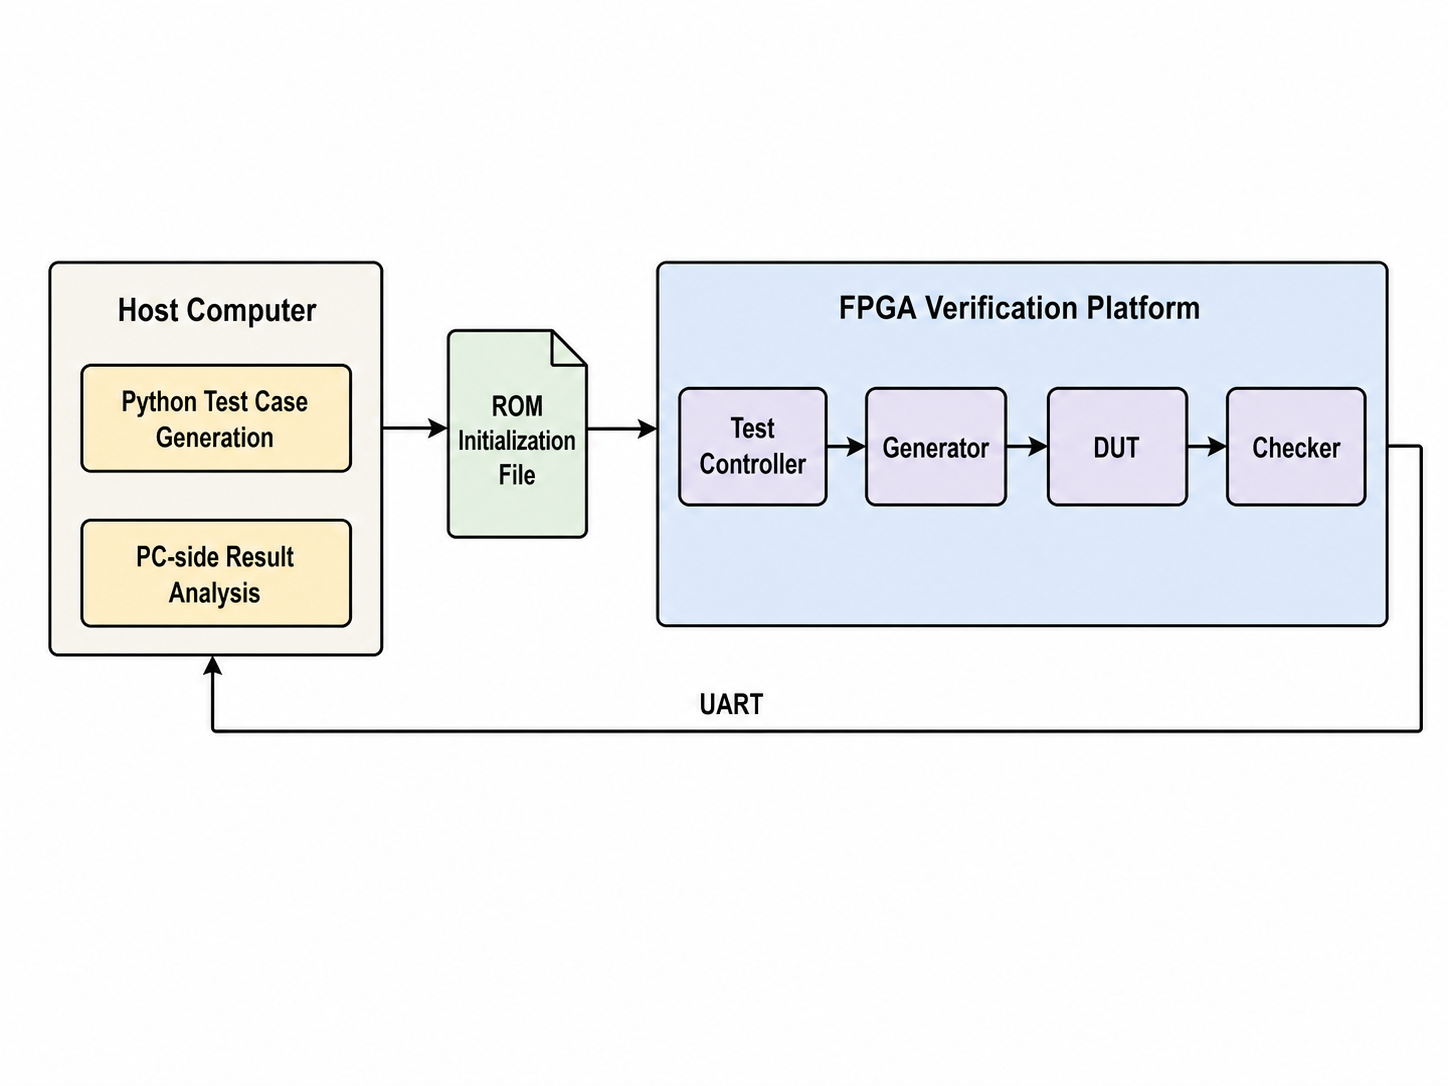
\includegraphics[width=0.9\textwidth]{images/ch4_verification_and_results/overall_platform.png}
    \caption{Overall verification platform}
    \label{fig:verification_platform}
\end{figure}


\subsection{Python-based Test Case Generation}
The Python side is responsible for generating the test cases before they are executed on the FPGA verification platform. Instead of embedding predefined test scenarios directly into the hardware test logic, the verification inputs are constructed on the host computer and then converted into a ROM initialization file. This makes the test cases easier to modify, reproduce, and extend.

In this verification flow, the test-generation scripts define the packet-level information used by the DUT, including the source node, destination node, packet length, start time, message type, and flit contents. The generated packets are first organized as structured test cases and are then encoded into a ROM initialization format. This ROM data is used to initialize the on-chip memory before FPGA execution, allowing the FPGA-side controller to read predefined packet entries during the test.

This method separates test construction from the hardware verification logic. New packet sequences can be generated by modifying the Python case definitions, while the FPGA-side controller, generator, and checker can remain unchanged. Therefore, the same hardware verification platform can be reused for different test scenarios, such as single-flit packets, concurrent packet injection, multi-flit packets, and larger repeated test sets.

Overall, Python-based test case generation provides a flexible and reproducible way to prepare verification inputs. It allows complex packet scenarios to be described at a higher level, encoded automatically, and executed by the FPGA-side verification platform without changing the DUT or the on-chip test logic.

\subsection{FPGA-based Verification Platform}
The FPGA-side verification platform is responsible for executing the generated test cases, injecting packets into the DUT, checking the received packets, and reporting the verification results. The platform is organized as an on-chip self-verification environment, where packet generation, packet checking, result buffering, and UART reporting are integrated into the FPGA logic.

The main modules of the FPGA-side verification platform are organized as follows:

\begin{itemize}
    \item \texttt{fpga\_board\_top}: Serves as the top-level wrapper for FPGA implementation. It connects the verification platform to board-level resources such as clock, reset, UART, and status signals.

    \item \texttt{fpga\_test\_controller}: Reads predefined packet entries from the initialized ROM and controls the execution of test cases. It schedules packet injection according to the packet start time and provides packet information to the generator.

    \item \texttt{fpga\_mesh\_traffic\_generator}: Converts packet entries into flits and injects them into the corresponding input ports of the DUT. It is responsible for generating valid packet streams according to the test schedule.

    \item \texttt{fpga\_mesh\_packet\_checker}: Observes the output side of the DUT and checks whether received packets match the expected results. It verifies destination, packet length, flit order, flit type, and related metadata, and produces packet-level pass/fail results.

    \item \texttt{fpga\_report\_fifo}: Buffers verification reports before UART transmission. This decouples the internal verification logic from the slower serial reporting interface.

    \item \texttt{fpga\_uart\_reporter}: Formats the verification reports and sends them to the host computer through UART for logging and further analysis.
\end{itemize}

\subsection{UART Reporting and PC-side Result Analysis}
UART is used as the reporting interface between the FPGA-side verification platform and the host computer. After packets are injected, checked, and classified on chip, the generated verification reports are sent through the UART interface. In this verification flow, UART is not part of the NoC data path; it is only used to transfer test results and status information to the PC.

The reported information includes packet-level and case-level events. Packet-level reports indicate whether an injected packet has been successfully received or failed due to an error condition. Case-level reports summarize the execution result of each test case, including pass/fail information and latency-related statistics. Progress and completion messages can also be returned to indicate the current execution state of the verification platform.

On the PC side, the received UART messages are recorded and parsed into structured result files. These results can then be used to analyze packet correctness, error distribution, and latency behavior. By moving result collection and analysis to the PC side, the FPGA logic only needs to perform essential checking and reporting, while more detailed statistical analysis can be handled after execution.

\subsection{Test Case Design}
The test cases are designed to cover both basic packet delivery and more complex communication situations in the $3 \times 3$ mesh NoC. Each case contains predefined packet information, including the source node, destination node, packet length, start time, message type, and flit contents. By changing these fields, different transmission scenarios can be generated and executed by the same FPGA-side verification platform.

The test set is organized into several case types:

\begin{itemize}
    \item \textbf{Single-flit basic case:} Verifies basic connectivity between source and destination nodes using head-tail packets. This case is used to check whether packets can be correctly injected, routed, received, and reported.

    \item \textbf{Concurrent single-flit case:} Injects multiple single-flit packets in overlapping time windows. This case is used to verify whether the NoC can handle simultaneous packet transmission and arbitration between competing requests.

    \item \textbf{Multi-flit packet case:} Uses packets containing head, body, and tail flits. This case checks whether flit order, packet length, and packet termination are handled correctly.

    \item \textbf{Mixed packet case:} Combines multiple packets with different lengths, message types, source-destination pairs, and injection times. This case is used to evaluate more general packet movement and interaction between different packets.
\end{itemize}

A repeat mechanism is also used to increase the number of executed cases. By repeating selected case types, the verification scale can be enlarged without changing the FPGA-side verification logic. This helps expose errors that may not appear in small directed tests and provides more data for latency and correctness analysis.



\chapter{Discussion and Future Work}
\label{ch5:discussion_and_future_work}



%%%%%%%%%%%%%%%%%%
\appendix %   <------
%%%%%%%%%%%%%%%%%%
\label{ap:ap1}
\cleardoublepage
\phantomsection
\chapter*{References}
\addcontentsline{toc}{chapter}{References}
\printbibliography[heading=none]
\end{document}
